\makeheading{Lecture 20 | 2020-11-18}
\section{Combining Cross Validation With Model Selection}
\begin{itemize}
    \item Given some candidate models (e.g., with different
          variables included) we can do $ K $-fold
          cross-validation using each of them, and choose the one
          with the lowest average prediction error across
          the folds, e.g., $ \displaystyle
              \frac{1}{K} \sum_{k=1}^{K} \text{RSME}_k $.
    \item How to choose $ K $? Some common choices are:
          \begin{itemize}
              \item $ K=5 $
              \item $ K=10 $
              \item $ K=N $ (number of observations for train/valid).
                    This is commonly known as ``leave one out'' (LOO).
          \end{itemize}
          The more folds, the higher the computational time, but
          it can give a better estimate of prediction error.
    \item What if we are not given a list of models to compare?
          (and if there are too many predictors to do all possible
          regressions). Then, we can combine cross-validation with
          \emph{model selection procedures} (criteria based on training
          data and search strategy).
\end{itemize}
To estimate the prediction error for a given
\emph{model selection procedure} we apply it $ K $ times,
each time treating observations in fold $ 1,2,\ldots,K $
as validation sample, e.g., use the \emph{average}
RMSE and choose the model selection procedure
with the lowest estimated prediction error.

\underline{Note}: actual variables selected in each fold might
be different.

\underline{Recommendation}: apply chosen
model selection \emph{procedure} (lowest estimated prediction error)
to the entire set of observations available for training
and validation to get a final model (for applications
to test data).

Recall we have:
\begin{itemize}
    \item $ \text{AIC}=2q-2\ln[L(\hat{\theta})] $
    \item $ \text{BIC}=q\ln(n)-2\ln[L(\hat{\theta})] $
\end{itemize}
We can go further (and beyond \emph{PLUS ULTRA!}) and consider the following.
\begin{Definition}{$ L_0 $ Penalized Likelihood}{}
    For any $ \lambda>0 $,
    \[ q\lambda -2\ln[L(\hat{\theta})] \]
\end{Definition}
\underline{Beyond Stepwise Regression}
\begin{itemize}
    \item Stepwise is a deterministic algorithm which is fast,
          but might not give optimal model selected.
    \item Could try stochastic algorithm, e.g., iterative
          conditional minimization (ICM)
\end{itemize}

\section{Iterative Conditional Minimization}
Start with a model with just intercept.
For a given random seed, take predictors $ x_1,\ldots,x_p $
and randomly re-order them into $ x_{(1)},\ldots,x_{(p)} $.
For $ j=1,\ldots,p $: (let $ \mathcal{S} $ be the predictors
currently in model, so start at $ \mathcal{S}=\emptyset $).
\begin{itemize}
    \item If $ x_{(j)} $ is not in $ \mathcal{S} $:
          \begin{itemize}
              \item Fit model with $ \mathcal{S} $.
                    If addition of $ x_{(j)} $ improves criterion,
                    then add $ x_{(j)} $ to $ \mathcal{S} $.
          \end{itemize}
    \item If $ x_{(j)} $ is in $ \mathcal{S} $:
          \begin{itemize}
              \item Fit model removing $ x_{(j)} $. If excluding
                    $ x_{(j)} $ improves criterion, then remove
                    $ x_{(j)} $ from $ \mathcal{S} $.
          \end{itemize}
\end{itemize}
Repeat for loop until no predictors are added/removed
from an entire pass through the for loop.
\begin{Remark}{}{}
    Different random orderings could give different
    sets $ \mathcal{S} $ at end of procedure, could pick one
    that has the best criterion overall.
\end{Remark}
\subsection{R Demo}
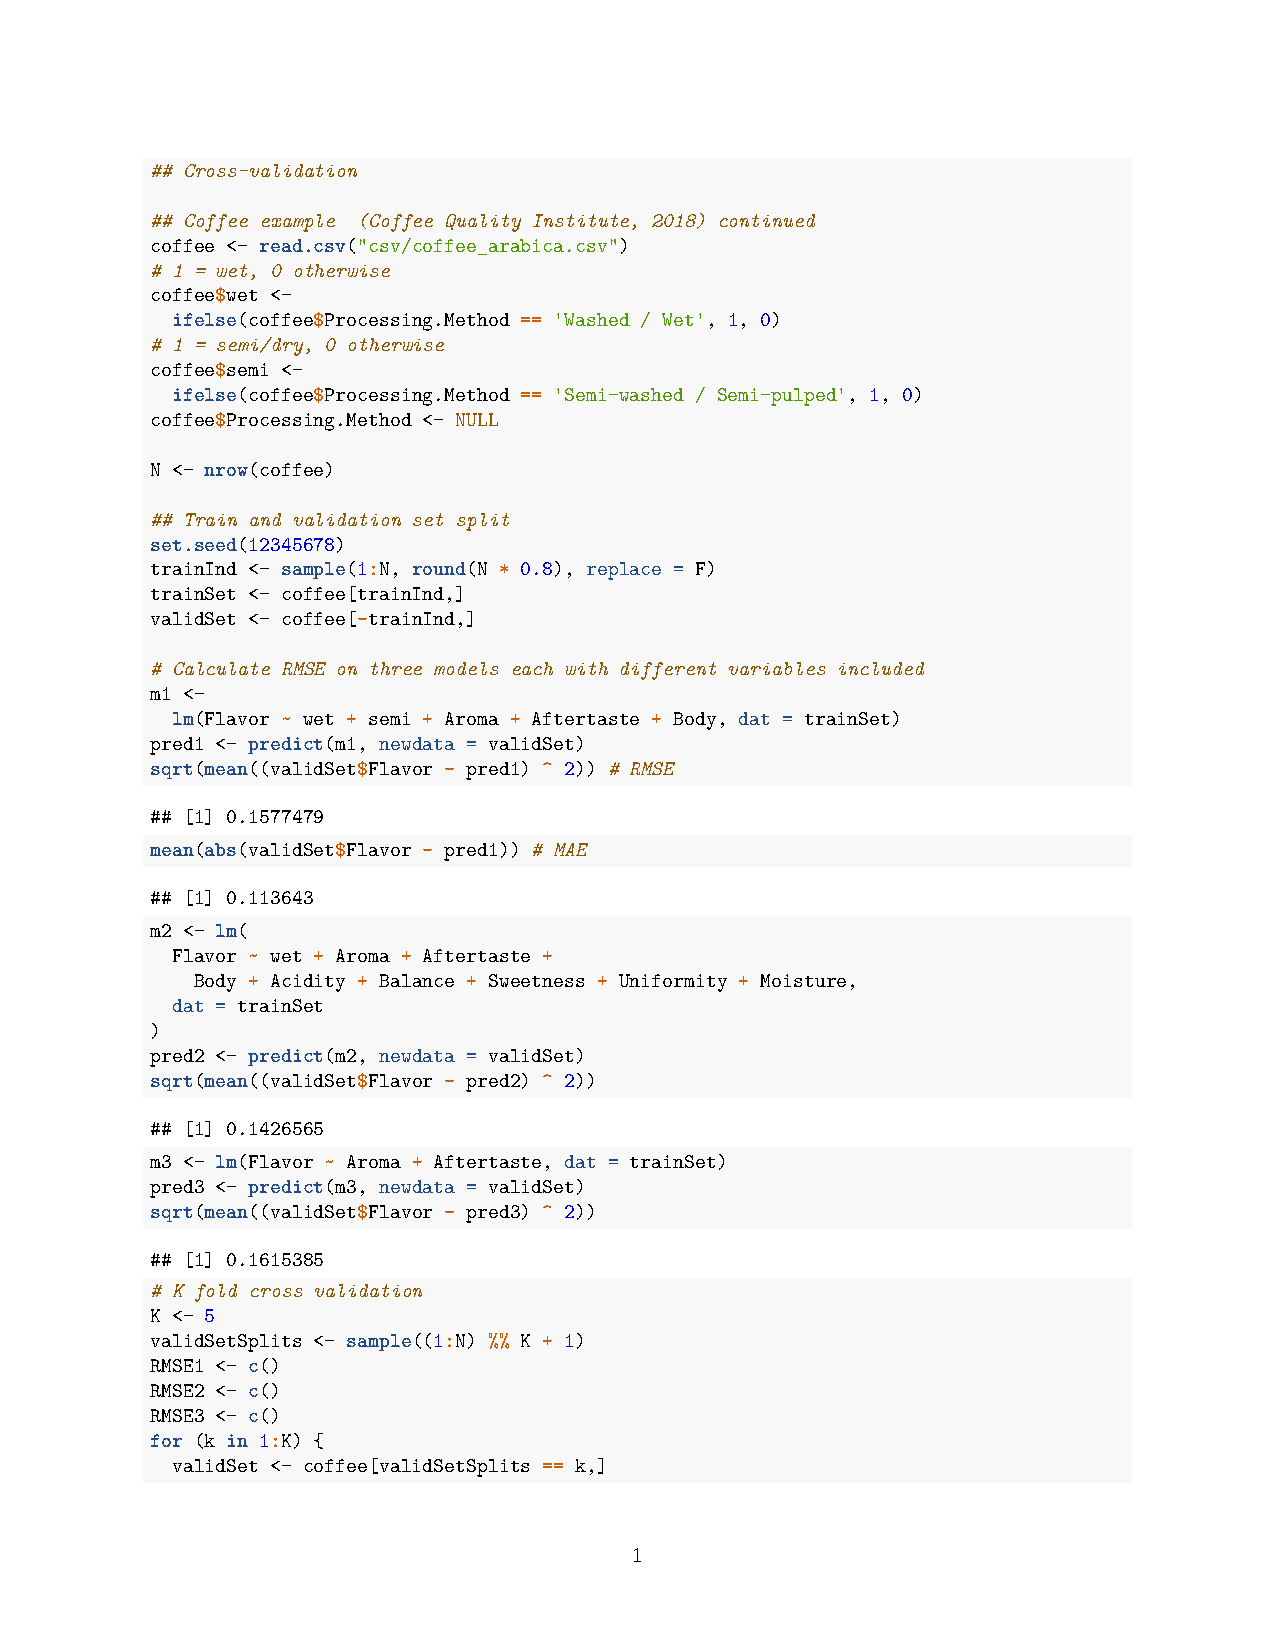
\includepdf[pages=-]{lec_19-demo.pdf}
